\documentclass{article}
\usepackage[T1]{fontenc}
\usepackage[utf8]{inputenc}

\usepackage{xspace}
\usepackage{graphicx}
\usepackage{amsmath}
\usepackage{amsfonts}
\usepackage{subfig}
\usepackage{fullpage}
\usepackage{url,paralist}
\usepackage{caption}

\author{Philip Pickering\\ \url{pgpick@gmx.at} \and Marco Eilers\\ \url{eilers.marco@googlemail.com} \and Thomas Bracht Laumann Jespersen\\ \url{ntl316@alumni.ku.dk}}
\title{Statistical Methods for Machine Learning\\ Assignment 2: Basic Learning Algorithms}
\date{}

\newcommand{\vect}[1]{\ensuremath{\boldsymbol{\mathbf{#1}}}\xspace}

%% For readability in question 1.3
\newcommand{\Target}{\vect{\mathsf{T}}}
\newcommand{\vPhi}{\vect{\Phi}}
\newcommand{\vw}{\vect{w}}
\newcommand{\Szero}{\vect{S}_0}
\newcommand{\mzero}{\vect{m}_0}
\newcommand{\target}{\vect{\mathsf{t}}}

\newcommand{\knollA}{\textsc{knollA}\xspace}
\newcommand{\knollB}{\textsc{knollB}\xspace}
\newcommand{\knollC}{\textsc{knollC}\xspace}

%% %% Uncomment these lines to get a box around all figures
%% \usepackage{float}
%% \floatstyle{boxed}
%% \restylefloat{figure}

\begin{document}
\maketitle

\section{Regression}

\subsection{Maximum Likelihood solution}

We are using a linear model:
\[
y(\vect{x},\vect{w}) = w_0 + w_1 x_1 + w_2 x_2 + \dots + w_D x_D
\]
and we let $\phi_i(\vect{x}) = x_i$ for $i = 1,\dots,D$ and
$\phi_0(\vect{x}) = 1$.

\subsubsection{Selection 1}

For our first selection $S_1$ our design matrix becomes a $200\times
5$ matrix.

\[
\vect{\Phi}_{S_1} = \begin{bmatrix}1 & \vect{x}_{1,1} & \vect{x}_{1,2} & \vect{x}_{1,3} & \vect{x}_{1,4}\\
\hfill & \hfill & \vdots & \hfill & \hfill\\
1 & \vect{x}_{i,1} & \vect{x}_{i,2} & \vect{x}_{i,3} & \vect{x}_{i,4}\\
\hfill & \hfill & \vdots & \hfill & \hfill\\
1 & \vect{x}_{N,1} & \vect{x}_{N,2} & \vect{x}_{N,3} & \vect{x}_{N,4}\\
\end{bmatrix}
\]
where the notation $\vect{x}_{i,j}$ indicates the $j$'th entry in the
$i$'th vector. %%Similarly we obtain a design matrix for our second
%%selection, $S_2$ of dimensions $200\times 2$, with $D = 2$:

Finding the ML estimate of our parameters for $S_1$ gives
\[
\vect{w}_{S_1} = \left[\!\begin{tabular}{r@{.}l} -43 & 0947\\ -0 &
  1299\\ 0 & 0352\\ 0 & 9335\\ -0 &
  0433\end{tabular}\!\right]\quad\text{ and }\quad \mathrm{RMS}_{S_1} = 4.3897
\]

\subsubsection{Selection 2}

Our second selection $S_2$ consists only of the data from the `Abdomen
2' column, giving a design matrix $\vect{\Phi}_{S_2}$ of dimensions
$200\times 2$. Training the model on the same training data yields:
\[
\vect{w}_{S_2} = \left[\!\begin{tabular}{r@{.}l}
  -37 & 4085\\
  0 & 6133
  \end{tabular}\!\right]\quad
\text{ and }\quad \mathrm{RMS}_{S_2} = 5.2064
\]

%% Conclusion
\subsubsection{Discussion}
Just looking at the root mean square values of the two selections, it
appears that $S_1$ performs better than $S_2$, but not by a lot. This
could suggest that either the variable `Abdomen 2' is the most descriptive
in terms of body fat, or that the linear model simply is a poor fit no
matter how many variables we include. It could be a combination of the
two.

It could probably be argued that the linear regression model is a poor
predictor, but including more variables should improve the results.

\subsection{Maximum a posteriori solution}

%% Use MAP estimation. Fix prior to zero mean isotropic Gaussian (eq. 3.52)
%% \[
%% p(\vect{w}|\alpha) = \mathcal{N}(\vect{w}|\vect{0},\alpha^{-1}\vect{I})
%% \]
%% Set noise precision parameter $\beta = 1$. Compute (3.53) and (3.54)
%% \[
%% \text{(3.53)}\quad \vect{m}_N = \beta\vect{S}_N\vect{\Phi}^T\mathsf{t}
%% \]
%% and
%% \[
%% \text{(3.54)}\quad \vect{S}_N^{-1} = \alpha\vect{I} + \beta\vect{\Phi}^T\vect{\Phi}
%% \]

\begin{figure}
\subfloat[\hfill]{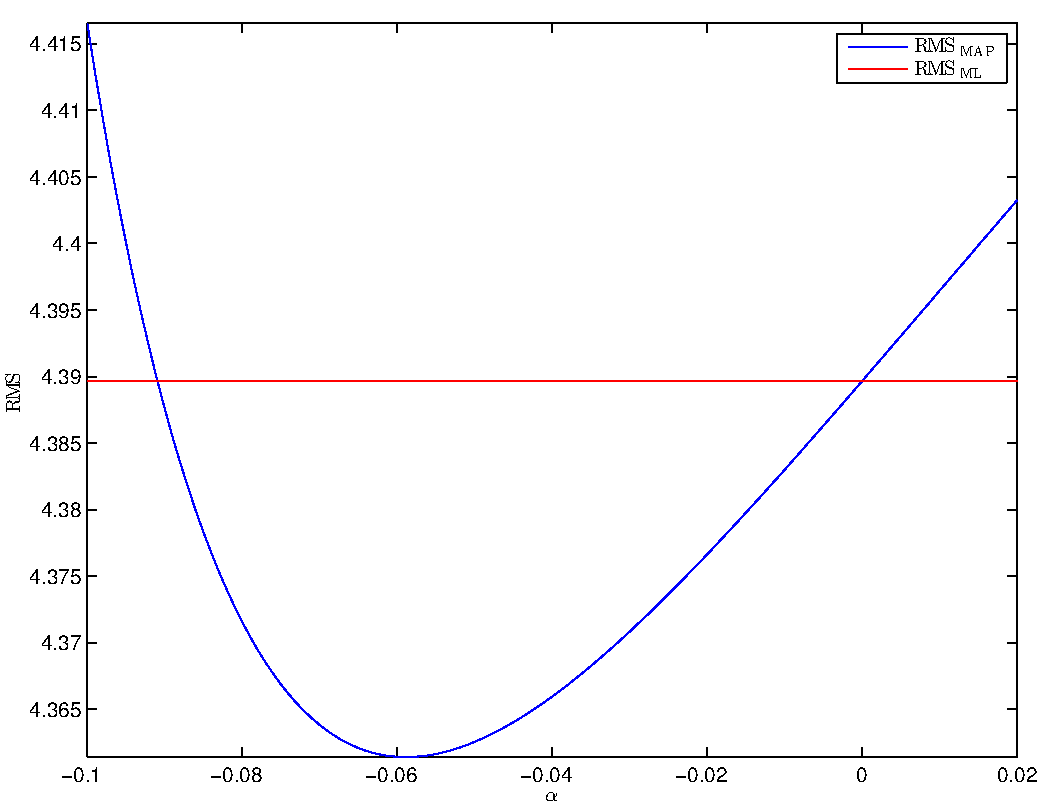
\includegraphics[width=.5\textwidth]{src/mapsel1.pdf}}
\subfloat[\hfill]{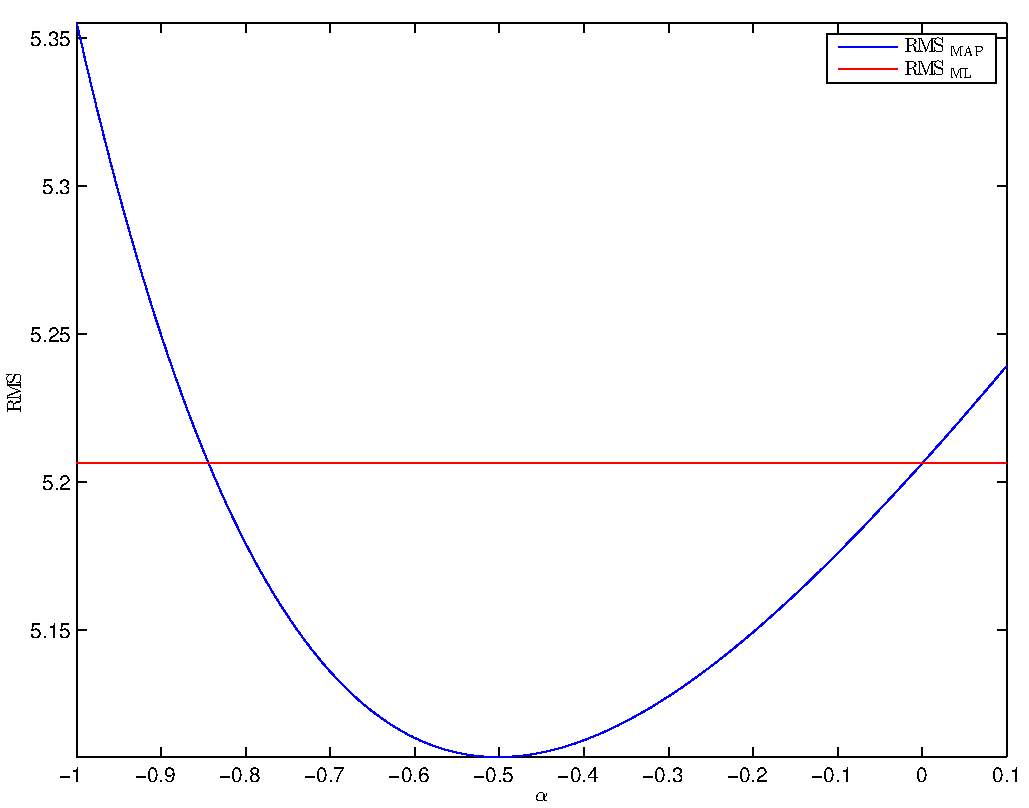
\includegraphics[width=.5\textwidth]{src/mapsel2.pdf}}
\caption{Plot of RMS against varying values of $\alpha$}
\label{fig:rmsalpha}
\end{figure}

For $S_1$ the lowest root mean square value is 4.3614, the same as the
ML solution differing on the second digit. The difference is larger
for $S_2$ in which we obtain the value 5.1071, differing from the ML
solution on the first digit.

In fig.~\ref{fig:rmsalpha} two plots are found of the root mean square
values for varying values of $\alpha$. In both plots we set $\beta =
1$. The RMS value of the ML solution is plotted as a straight line.

%%Apply model to test set and compute RMS error for different values of the precision parameter $\alpha$.

\subsubsection{Comparison}

Firstly, we can observe for both plots that when $\alpha = 0$, we
obtain the same $\mathrm{RMS}$ error for the MAP estimate as for the
ML solution. This is expected and demonstrates that when our prior
precision parameters are set to zero, the MAP estimate becomes the ML
estimate.

Fig.~\ref{fig:rmsalpha}(a) is the plot for $S_1$, and it can be seen
that the $\mathrm{RMS}_\mathrm{MAP}$ error drops below the
$\mathrm{RMS}_\mathrm{ML}$ in the interval $[-0.091,0]$. In
fig.~\ref{fig:rmsalpha}(b) the plot for $S_2$ similarly gives us that
the $\mathrm{RMS}_\mathrm{MAP}$ error is lower in the interval
$[-0.844,0]$.

The intervals in which the MAP estimate outperforms the ML estimate
are very small, and the obtained difference likewise small.

\newpage
\subsection{Theory}

We have from CB (1.44) that:
\[
p(\vect{w}|\vect{\mathsf{t}}) \propto p(\vect{\mathsf{t}}|\vect{w})\times p(\vect{w}),
\]
which reads that the probability distribution of the parameters given
the target vector $\vect{\mathsf{t}}$ is proportional to the
probability of the target vector given the parameters multiplied by
the probability of the parameters.

This is also Bayes' Theorem in words, namely the posterior
distribution is proportional to the likelihood times the prior.

With this in mind we state the likelihood function defined in CB
(3.10)
\begin{align*}
  p(\target |\vect{X}, \vect{w}, \beta) &= \prod_{n=1}^N \mathcal{N}(t_n | \vect{w}^T\vect{\phi}(\vect{x}_n), \beta^{-1})\label{eq:likelihood}\\
%%  \intertext{which we know from the lecture slides can be written as}
  &= \mathcal{N}(\vect{\mathsf{T}} | \vect{\Phi}\vect{w}, \beta^{-1}\vect{I}) \qquad\text{(from the lecture slides)}
\end{align*}
and the prior is given by:
\[
  p(\vect{w}) = \mathcal{N}(\vect{w}|\vect{m}_0,\vect{S}_0).
\]

As is written in CB page 153, the product of the two Gaussians will
again be Gaussian, but we want to verify the result of the
multiplication, so we want to `complete the square' in the
exponential. In order to verify the result we would then need to find the normalization coefficient using the
standard result for a normalized Gaussian.

\begin{align}
  \nonumber  & \exp\left\{-\frac{1}{2}(\Target - \vPhi\vw)^T \beta\vect{I} (\Target -
  \vPhi\vw)\right\} \times \exp\left\{ -\frac{1}{2}(\vw -
  \mzero)^T\Szero^{-1}(\vw - \mzero)\right\}\\
  \nonumber = & \exp\left\{-\frac{\beta}{2}(\Target - \vPhi\vw)^T (\Target -
  \vPhi\vw)\right\} \times \exp\left\{ -\frac{1}{2}(\vw -
  \mzero)^T\Szero^{-1}(\vw - \mzero)\right\}\\
  = & \exp\left\{-\frac{\beta}{2}(\Target - \vPhi\vw)^T (\Target -
  \vPhi\vw) -\frac{1}{2}(\vw - \mzero)^T\Szero^{-1}(\vw - \mzero)\right\}\label{eq:expgauss}
\end{align}

Multiplying out the expression in \eqref{eq:expgauss} we find (excluding the exp part):
\begin{align}
  %%= & -\frac{\beta}{2}(\Target - \vPhi\vw)^T (\Target - \vPhi\vw) -\frac{1}{2}(\vw - \mzero)^T\Szero^{-1}(\vw - \mzero)\right\}\\
\nonumber = & -\frac{1}{2}\left(\beta\Target^T\Target - \beta\Target\vPhi\vw - \beta\vw^T\vPhi^T\Target + \beta\vw^T\vPhi^T\vPhi\vw + \vw^T\Szero^{-1}\vw - \vw^T\Szero^{-1}\mzero - \mzero^T\Szero^{-1}\vw + \mzero^T\Szero^{-1}\mzero \right)\\
\intertext{Rearranging in terms of \vw and $\vw^T$ gives us:}
= & -\frac{1}{2}\left(\vw^T(\beta\vPhi^T\vPhi + \Szero^{-1})\vw - \vw^T(\beta\vPhi^T\Target + \Szero^{-1}\mzero) - (\beta\Target^T\vPhi + \mzero^T\Szero^{-1})\vw + \mzero^T\Szero^{-1}\mzero + \beta\Target^T\Target \right)\label{eq:sqalmostcomplete}
\end{align}
The last two terms in \eqref{eq:sqalmostcomplete} we can ignore, because they are independent of \vw and we will treat them as constant. The expression can be simplified if we set $\vect{A} = \beta\vPhi^T\vPhi + \Szero^{-1}$ and $\vect{B} = \beta\vPhi^T\Target + \Szero^{-1}\mzero$. We also make use of the fact that $(\beta\Target^T\vPhi + \mzero^T\Szero^{-1}) = (\beta\vPhi^T\Target + \Szero^{-1}\mzero)^T = \vect{B}^T$, i.e.\ that $\Szero$ is symmetric, and correspondingly for its inverse it holds that $(\Szero^{-1})^T = \Szero^{-1}$.
\begin{align*}
  \eqref{eq:sqalmostcomplete} &= -\frac{1}{2}\left(\vw^T\vect{A}\vw - \vw^T\vect{B} - \vect{B}^T\vw \right)\\
  & = -\frac{1}{2}(\vw - \vect{A}^{-1}\vect{B})^T\vect{A}(\vw - \vect{A}^{-1}\vect{B})\\
\intertext{from which we can clearly see that $\vect{S}_N^{-1} = \vect{A}$ and $\vect{m}_N = \vect{A}^{-1}\vect{B} = \vect{S}_N(\beta\vPhi^T\vPhi + \Szero^{-1})$}
& = -\frac{1}{2}(\vw - \vect{m}_N)^T\vect{S}_N(\vw - \vect{m}_N)
\end{align*}
which is the result that we wanted. Note also we've made use of the fact that $\vect{S}_N$ is symmetric. This is true because $\vPhi^T\vPhi$ and $\Szero^{-1}$ both are symmetric and any given linear combination of symmetric matrices will itself be symmetric.


\newpage
\section{Linear Discriminant Analysis}
\begin{figure}
  \subfloat[\knollA]{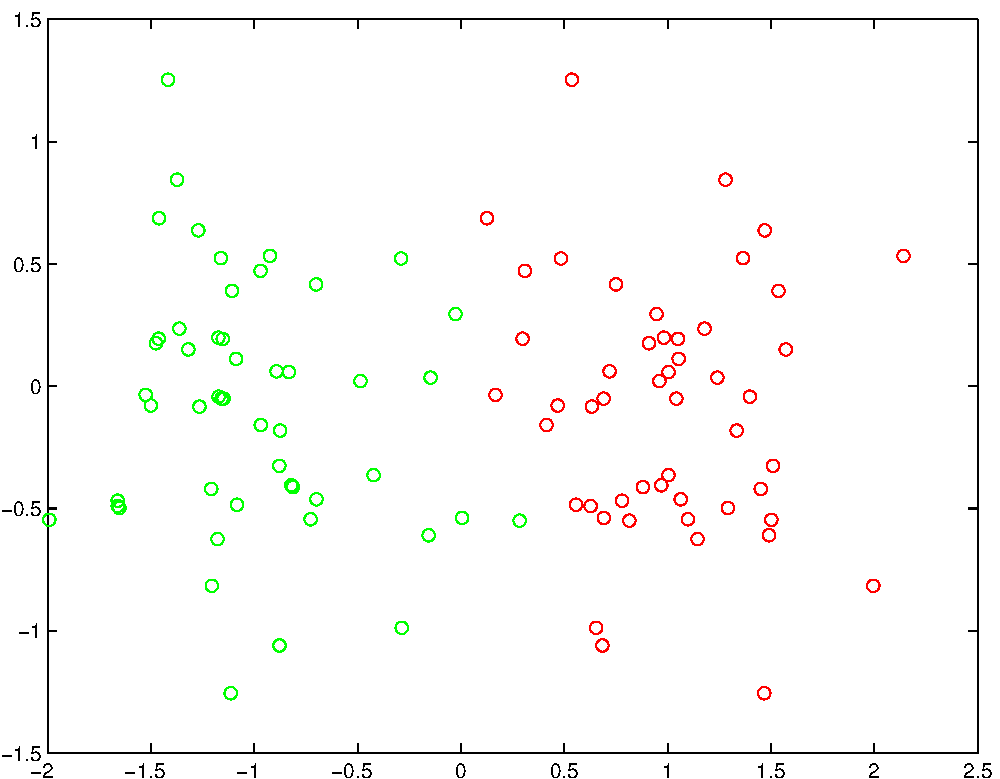
\includegraphics[width=.33\textwidth]{src/knollAtrain.pdf}}
  \subfloat[\knollB]{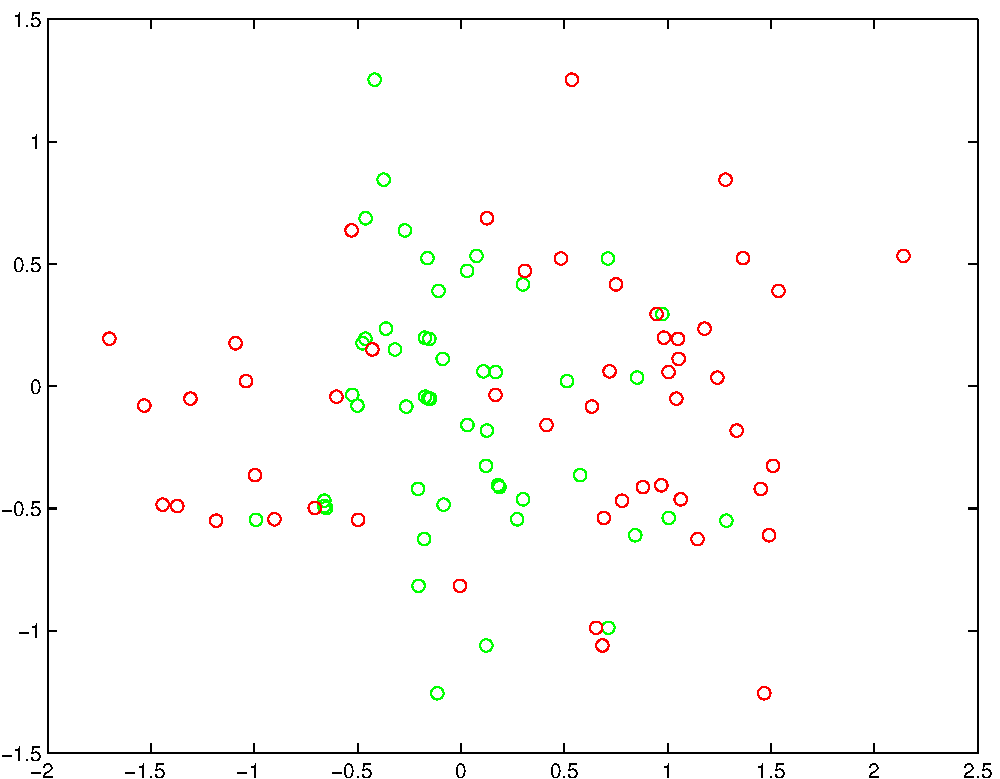
\includegraphics[width=.33\textwidth]{src/knollBtrain.pdf}}
  \subfloat[\knollC]{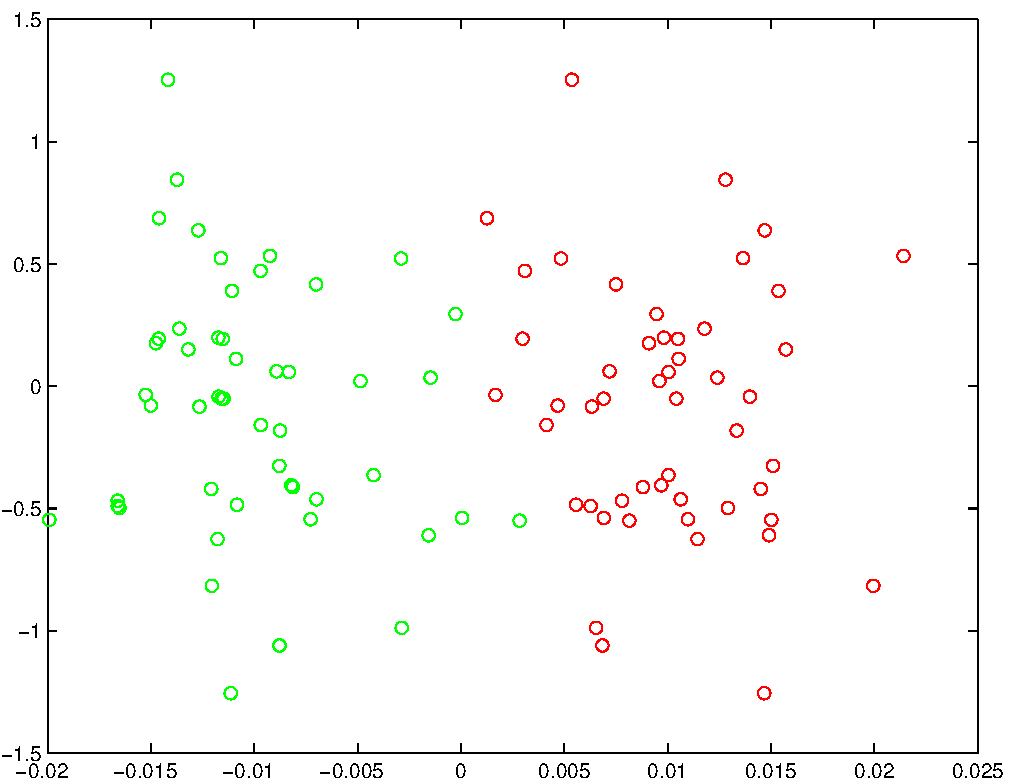
\includegraphics[width=.33\textwidth]{src/knollCtrain.pdf}}
  \caption{Visualisation of the training data for each of the \textsc{knoll} problems}
  \label{fig:knolldata}
\end{figure}

\subsection{Observations regarding the data}
\begin{figure}

  \subfloat[\hfill]{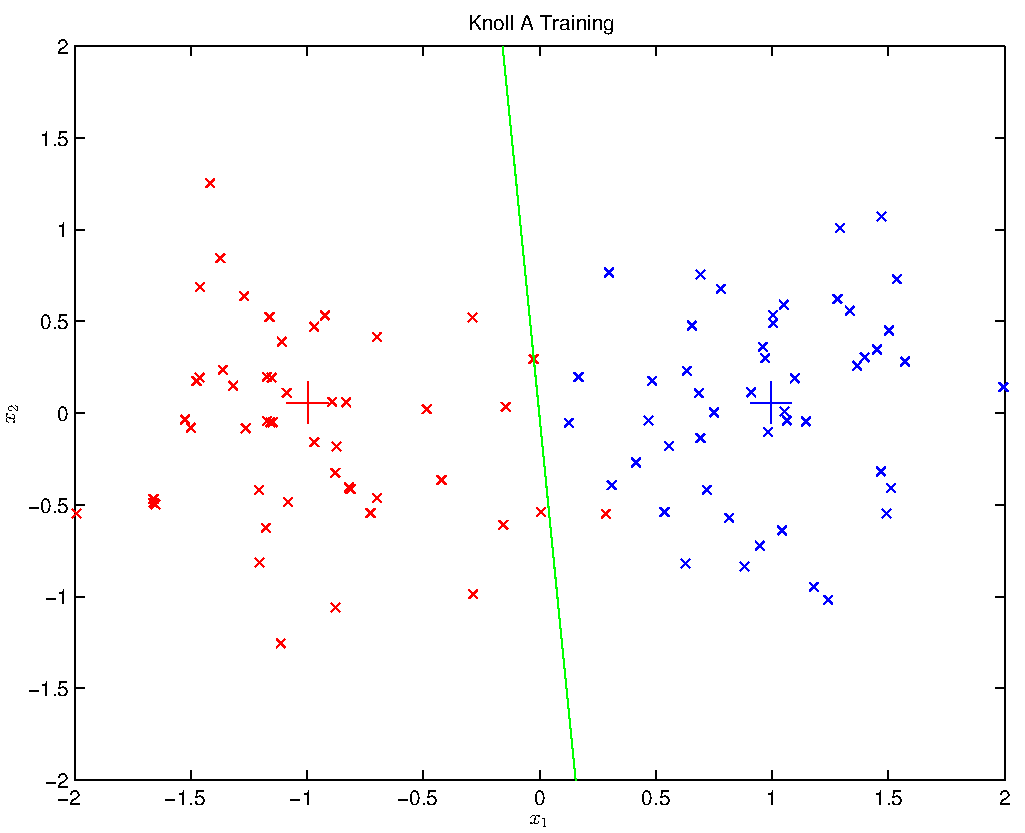
\includegraphics[width=.5\textwidth]{src/ldaKnollAtrain.pdf}}
  \subfloat[\hfill]{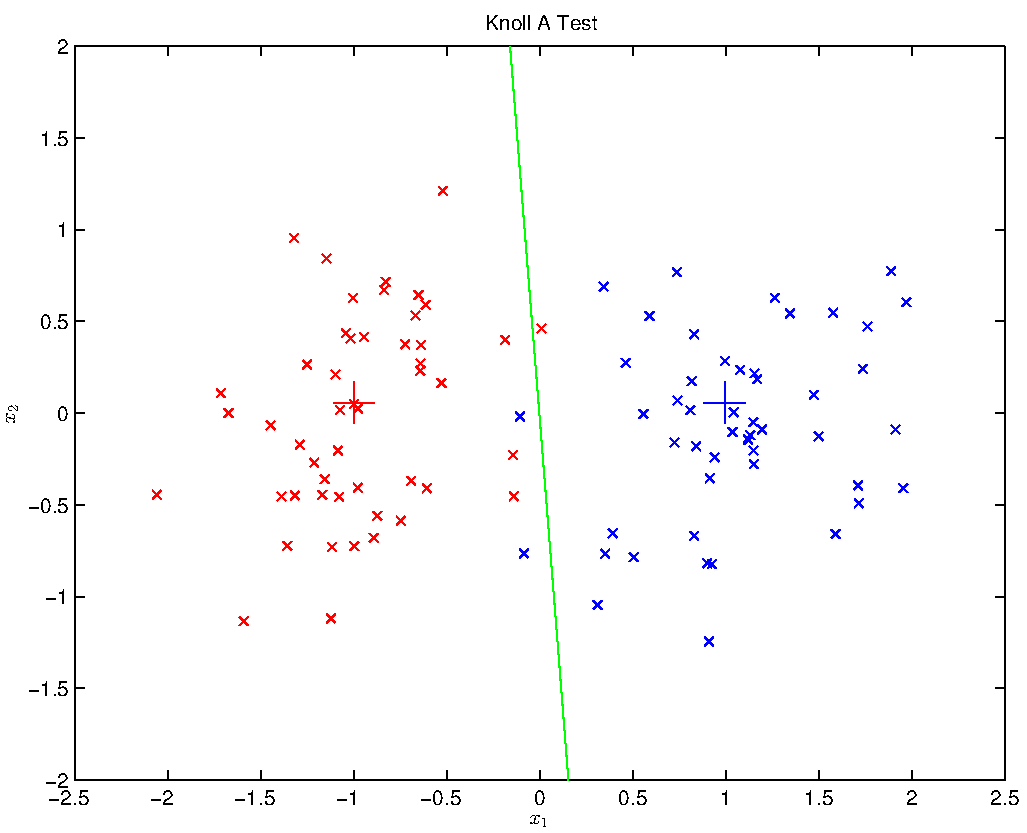
\includegraphics[width=.5\textwidth]{src/ldaKnollAtest.pdf}}

  \subfloat[\hfill]{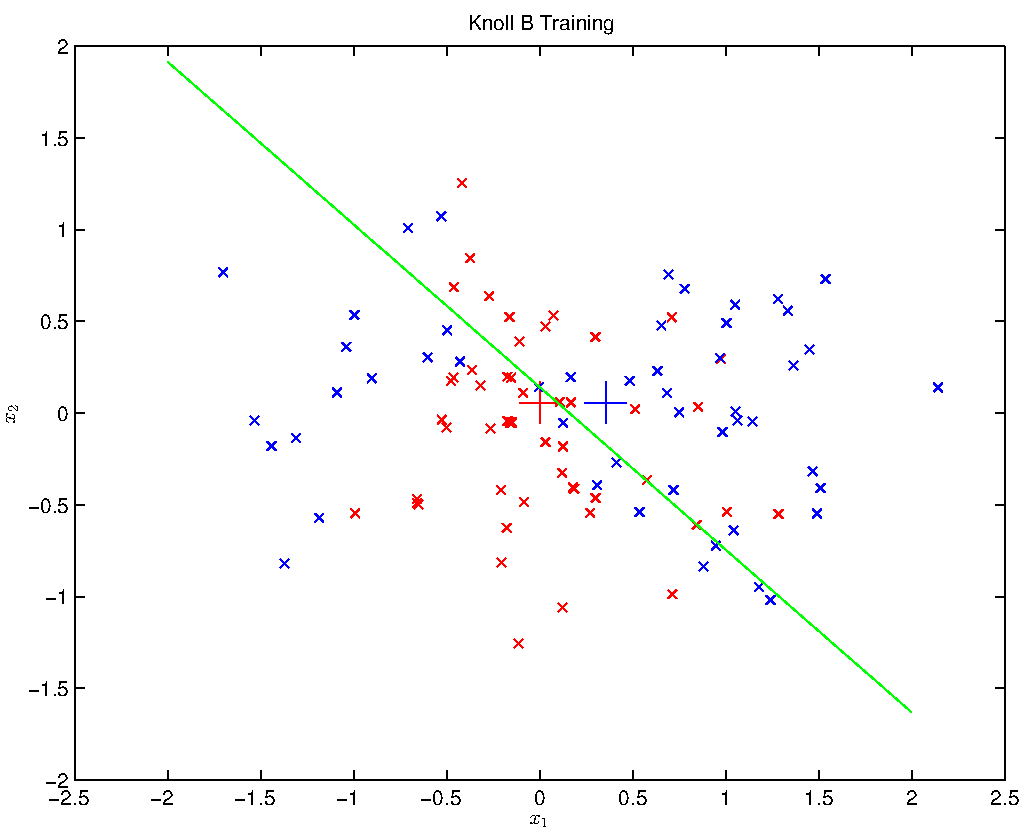
\includegraphics[width=.5\textwidth]{src/ldaKnollBtrain.pdf}}
  \subfloat[\hfill]{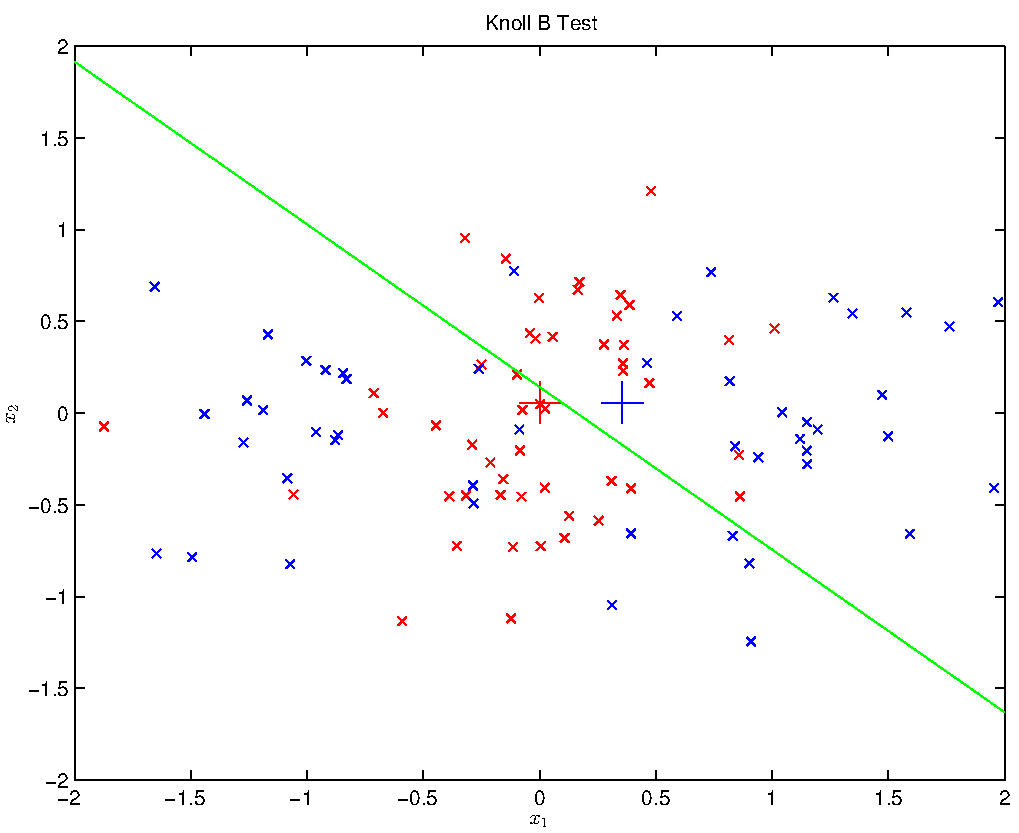
\includegraphics[width=.5\textwidth]{src/ldaKnollBtest.pdf}}

  \subfloat[\hfill]{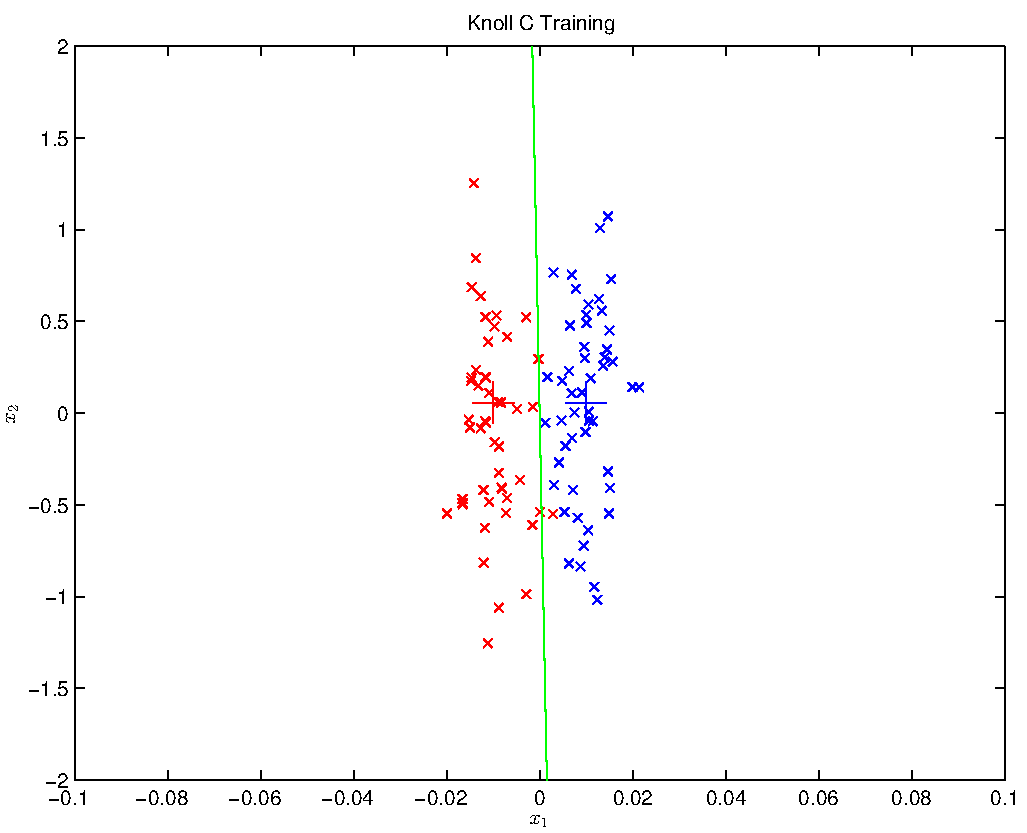
\includegraphics[width=.5\textwidth]{src/ldaKnollCtrain.pdf}}
  \subfloat[\hfill]{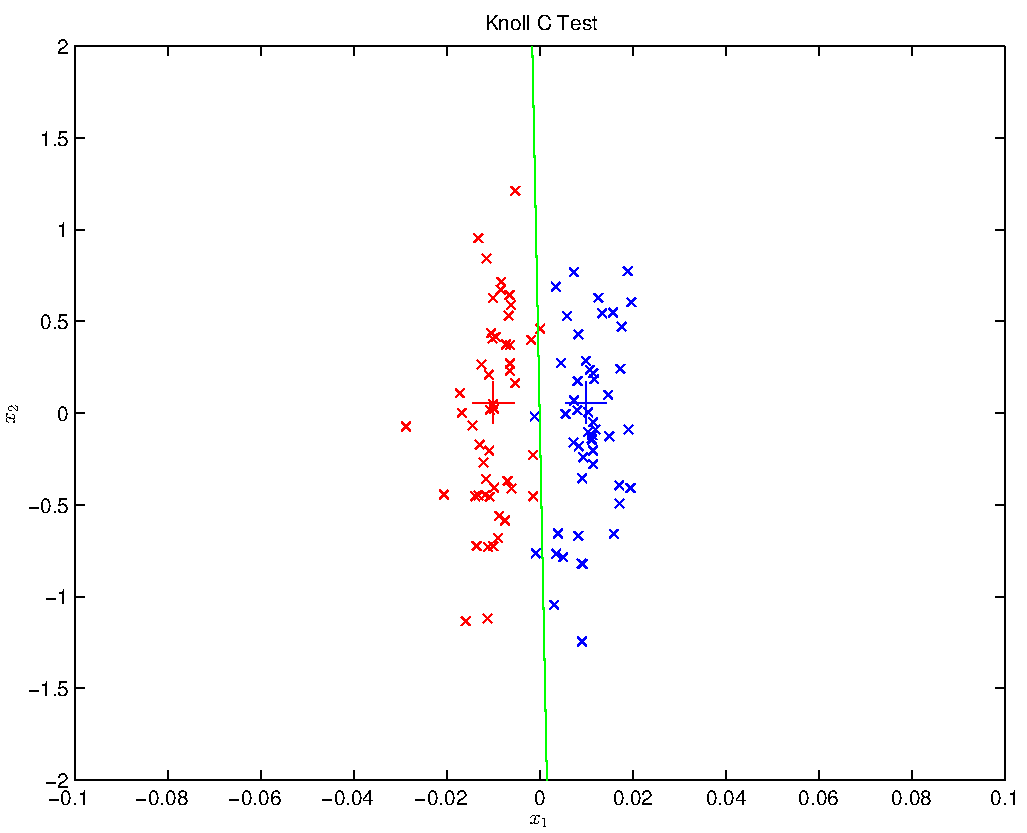
\includegraphics[width=.5\textwidth]{src/ldaKnollCtest.pdf}}

  \caption{Visualisation of the training data for each of the \textsc{knoll} problems}
  \label{fig:ldaknollplots}
\end{figure}

In fig.~\ref{fig:knolldata} you can see plots of all three training data sets. It is obvious
that while \knollA and \knollC contain well-separable groups of data points, the distributions in \knollB
seem to overlap. We can therefore expect that LDA will perform relatively well on \knollA and \knollB, whereas
the results for \knollB will likely be more erratic. 

\subsection{Results of LDA}
If we run LDA on all three data sets and plot them with their respective decision boundaries (fig.~\ref{fig:ldaknollplots}), we find 
that the algorithm indeed performs well on the \knollA and \knollC sets. In table~\ref{tab:ldaknollerror} we can see that although the error count is greater than zero for all 
training and test sets, which is also implied by the margin always being slightly negative, the number of errors
is relatively low for both training and test sets. The training set performs slightly better than the test set in both 
cases, which is to be expected, but there is not over- or underfitting problem.

For \knollB, however, the results are much worse. The properties of the underlying distribution simply
do not allow them to be separated by a straight line, which results in a high error percentage and a highly negative margin.

Since the distributions in \knollB overlap to a high degree, it is generally not possible to find a function of any kind
to separate both classes accurately. However, a Quadratic Discriminant Analysis might be able to adapt to the fact that one class
is more concentrated in $-0.5 \leq x_1 \leq 0.5$, whereas the other one has a higher variance and is therefore spread out more widely.
It could therefore assign all points in this range to one class and the rest to the other. While this will still result in a high
error percentage, such an algorithm might find the Bayes Optimal Solution or a good approximation.

\begin{table}[h!]
  \centering
  \begin{tabular}{l|c|c|c|c|c|c}
    & \multicolumn{2}{c|}{\knollA} & \multicolumn{2}{|c|}{\knollB} & \multicolumn{2}{|c}{\knollC} \\
    & Training & Test & Training & Test & Training & Test \\
    \hline
    Errors & 0.01 & 0.03 & 0.40 & 0.49 & 0.01 & 0.03 \\ 
    Margin & -0.242763 & -0.142026 & -1.629922 & -2.061411 & -0.002435 & -0.001425 \\
  \end{tabular}
  \caption{Error percentages and margins for each of the \textsc{knoll} problems}
  \label{tab:ldaknollerror}
\end{table}

\newpage
\section{Nearest Neighbor Classification}

\subsection{Nearest Neighbor Classification with Euclidian Metric}

The results of the runs of the classifier for different values of $k$
are found in table~\ref{tbl:results1}. The bottom field of each column
indicates the $k$ for which the classifier gave the lowest error rate.

The error rate is computed by adding up the errors made by the
classifier, and then dividing by the test set size. As we have the
actual class of a given point (for both test and training sets), this
is straightforward to implement.

As a general note, classifying the training set itself will always
give us $k = 1$ as the optimal value, which makes sense, because the
closest point to a point in both the training and test sets is the
point itself, hence the distance will always be zero (and the
classification perfect). But it's interesting to see how the
classifier behaves when more than one neighbor has to be
considered. If a point belonging to one class is surrounded by points
in the other class, then it will be misclassified. As can be seen from
the results, the optimal value for $k$ in all the training sets is $3$,
although it should be noted that the error rate for $k = 3,5$ and $7$
in \knollA are all $0.1$.

In \knollA, the error rates are very low ($< 0.05$) for all the values of $k$,
being lowest when $k = 3$. In \knollB and \knollC the error rates
increase dramatically ($\geq 0.19$), for \knollB the lowest error rates are obtained
when $k = 5$ or $7$. In \knollC the best results are unanimously
obtained when $k = 1$.

%% Hand in: classifier source code, results, short discussion.
%%% Table
%%% k    knollA    knollB    knollC
%%% 1      %                   %
%%% 3
%%% 5
%%% 7
%%% 9      %                   %
\begin{table}
  \centering
  \begin{tabular}{c | c|c | c|c | c|c}
    \hfill & \multicolumn{2}{c|}{\knollA} & \multicolumn{2}{c|}{\knollB} & \multicolumn{2}{c}{\knollC}\\
    $k$ & test & train & test & train & test & train\\\hline
    1 & 0.04 &   -  & 0.23 &   -  & 0.20 &   - \\
    3 & 0.02 & 0.01 & 0.20 & 0.13 & 0.32 & 0.16\\
    5 & 0.03 & 0.01 & 0.19 & 0.19 & 0.34 & 0.21\\
    7 & 0.04 & 0.01 & 0.19 & 0.19 & 0.42 & 0.21\\
    9 & 0.03 & 0.02 & 0.23 & 0.20 & 0.46 & 0.33\\\hline\hline
    \hfill & 3 & 3  &   5  &   3  &   1  &   3 
  \end{tabular}
  \caption{Table of error percentages for $k$-NN classifier on all three \textsc{knoll} problems.}
  \label{tbl:results1}
\end{table}

%% Why it makes sense to compute error rate for the training
We can compute an accuracy for the $k$-NN on the same training data, which for $k = 1$ always gives an error degree of zero, because the nearest neighbour of a given point in the data set is the point itself. But for higher values of $k$, we can get errors for points surrounded by points from the opposite class.

Both LDA and $k$-NN perform very well on \knollA, as would be expected because the points of the two classes seem cleanly separated in visualisation (fig.~\ref{fig:knolldata}). They also both perform quite bad on \knollB, but here $k$-NN outperforms LDA, because it only misclassifies about half as many points as does the LDA. This seems reasonable, because $k$-NN is able to to make use of the fact that the range of $-0.5 \leq x_1 \leq 0.5$ is more densely populated by points of one class, whereas outside of this range the other class is more dominant. This is the kind of distinction that cannot be achieved by a linear decision boundary.

On \knollC, on the other hand, LDA clearly outperforms $k$-NN, achieving near perfect results, while $k$-NN only performs about as good as it does for \knollB. The data in \knollC is such that the separation induced by a linear decision boundary gives a higher accuracy than just observing your $k$ nearest neighbours. In other words, a portion of the points lie so close to the decision boundary that they are geometrically closer to the points in the opposite class than points of their own class.

Another comment one could make in terms of computational performance, is that $k$-NN suffers from the fact that distances must be recomputed for every new point which for a large data set means a lot of computation. LDA has a overhead just in the training phase when computing $\vect{\mu}_1$, $\vect{\mu}_2$ and their common covariance \vect{\Sigma}---after that classification becomes simply a few multiplications and additions, which is nowhere near as computationally demanding as $k$-NN.

\subsection{Changing the Metric}

To prove that $d$ is a metric, given
\[
d(\vect{x},\vect{z}) = \|\vect{M}\vect{x} - \vect{M}\vect{z}\|\text{,
  where } \vect{M} = \begin{pmatrix} 100 & 0 \\ 0 & 1\end{pmatrix}
\]
and $\|\cdot\|$ is the standard $L_2$-norm (in $\mathbb{R}^2$), we
need to verify $\forall \vect{x},\vect{y}\in \mathbb{R}^2$ that
\begin{inparaenum}[1)]
  \item $d(\vect{x},\vect{y}) \geq 0$; 
  \item $d(\vect{x},\vect{y}) = 0 \Leftrightarrow \vect{x} = \vect{y}$;
  \item $d(\vect{x},\vect{y}) =  d(\vect{y},\vect{x})$ (symmetry) and
  \item $\forall \vect{x},\vect{y},\vect{z} \in \mathbb{R}^2 : d(\vect{x},z) \leq d(\vect{x},\vect{y}) + d(\vect{y},\vect{z})$.
\end{inparaenum}

\subsubsection{Proof}

We need only to observe that $\vect{M}$ is a projection $m : \mathbb{R}^2 \rightarrow \mathbb{R}^2$, i.e.\ onto $\mathbb{R}^2$ itself, given by $m(\vect{x}) = \vect{M}\vect{x}$. This immediately gives us all the properties we need, because $L_2$ is itself a (complete) metric on $\mathbb{R}^2$.

For instance, if we let $\vect{x},\vect{y},\vect{z} \in \mathbb{R}^2$ and $\vect{x'},\vect{y'},\vect{z'}$ be the result of applying $m$ on $\vect{x},\vect{y},\vect{z}$ respectively, we can prove the triangle inequality:

\begin{align}
\nonumber d(\vect{x},\vect{z}) &= \left\|\vect{M}\vect{x} - \vect{M}\vect{z}\right\|\\
\nonumber &= \left\|\vect{M}\vect{x} - \vect{M}\vect{y} + \vect{M}\vect{y} - \vect{M}\vect{z}\right\|\\
\nonumber &= \left\|(\vect{x'} - \vect{y'}) + (\vect{y'} - \vect{z'})\right\|\\
\nonumber &\leq \left\|\vect{x'} - \vect{y'}\right\| + \left\|\vect{y'} - \vect{z'}\right\|\quad \text{(by property of } L_2 \text{ norm)}\\
  &= d(\vect{x},\vect{y}) + d(\vect{y},\vect{z})
\end{align}

%% \subsubsection{Original proof --- the long way}

%% Let $\vect{x}, \vect{y} \in \mathbb{R}^2$. As it is easier to consider
%% the square of the $L_2$ norm, we will do so:
%% \begin{align}
%% \nonumber  d(\vect{x},\vect{y})^2 &= \left\|\begin{pmatrix} 100 & 0\\ 0 & 1\end{pmatrix}\begin{pmatrix}x_1\\ x_2\end{pmatrix} - \begin{pmatrix}100 & 0\\ 0 & 1\end{pmatrix}\begin{pmatrix}y_1\\ y_2\end{pmatrix}\right\|^2 \\
%%       \nonumber &= \left\| \begin{pmatrix} 100(x_1 - y_1)\\ x_2 - y_2\end{pmatrix}\right\|^2\\
%% \nonumber          &= \begin{pmatrix} 100(x_1 - y_1)\\ x_2 - y_2\end{pmatrix}^T\begin{pmatrix} 100(x_1 - y_1)\\ x_2 - y_2\end{pmatrix}\\
%%             &= (100(x_1 - y_1))^2 + (x_2 - y_2)^2 \label{eq:c1}.
%% \end{align}

%% From \eqref{eq:c1} we observe that $(x_1 - y_1)^2 \geq 0$ and
%% similarly $(x_2 - y_2)^2 \geq 0$ for all values in $\mathbb{R}$, so
%% our first criteria for a metric is fulfilled. We also observe that if
%% $d(\vect{x},\vect{y}) = 0$ it implies $x_1 - y_1 = 0$ and $x_2 - y_2 =
%% 0$, which means that $x_1 = y_1$ and $x_2 = y_2$, thus $d$ fulfills
%% our second requirement for a metric.

%% Our requirement of symmetry requires a little more
%% investigation. Proceeding from \eqref{eq:c1}, we find
%% \begin{align}
%% \nonumber (100(x_1 - y_1))^2 + (x_2 - y_2)^2 &= 100^2(x_1^2 - 2x_1y_1 + y_1^2) + (x_2^2 - 2x_2y_2 + y_2^2)\\
%%   \nonumber &= 100^2(y_1^2 - 2y_1x_1 + x_1^2) + (y_2^2 - 2y_2x_2 + x_2^2)\\
%%   \nonumber &= (100(y_1 - x_1))^2 + (y_2 - x_2)^2\\
%%   &= d(\vect{y},\vect{x})^2\label{eq:c2},
%% \end{align}
%% where \eqref{eq:c2} gives us $d(\vect{x},\vect{y}) =
%% d(\vect{y},\vect{x})$ and therefore fulfills the symmetry
%% requirement.

%% Our last requirement is the triangle inequality, i.e.\ $d(\vect{x},\vect{z}) \leq d(\vect{x},\vect{y}) + d(\vect{y},\vect{z}), \forall \vect{x},\vect{y},\vect{z}\in \mathbb{R}^2$.

%% Let $\vect{x},\vect{y},\vect{z}\in\mathbb{R}^2$.
%% \begin{align}
%%   d(\vect{x},\vect{z}) &= \left\|\vect{M}\vect{x} - \vect{M}\vect{z}\right\|\\
%%   &= \left\|\vect{M}\vect{z} - \vect{M}\vect{y} + \vect{M}\vect{y} - \vect{M}\vect{z}\right\|\\
%%   &\leq \left\|\vect{M}\vect{z} - \vect{M}\vect{y}\right\| + \left\|\vect{M}\vect{y} - \vect{M}\vect{z}\right\|\\
%%   &= d(\vect{x},\vect{y}) + d(\vect{y},\vect{z})
%%   %% &= (\vect{M}\vect{x} - \vect{M}\vect{z})^T(\vect{M}\vect{x} - \vect{M}\vect{z})\\
%%   %% &= ((\vect{M}\vect{x})^T - (\vect{M}\vect{z})^T)(\vect{M}\vect{x} - \vect{M}\vect{z})\\
%%   %% &= (\vect{M}\vect{x})^T\vect{M}\vect{x} \\
%%   %% &= \quad\vdots\quad \text{(We want to arrive at the following)} \\
%%   %% &\leq \left\|\vect{M}\vect{x} - \vect{M}\vect{y}\right\|^2 + \left\|\vect{M}\vect{y} - \vect{M}\vect{z}\right\|^2\\
%%   %% &= d(\vect{x},\vect{y})^2 + d(\vect{y},\vect{z})^2
%% \end{align}

\subsubsection{Results}
Using $d$ as metric on \knollC we obtain the results shown in table~\ref{tbl:knollCd}.

\noindent\begin{minipage}{.4\textwidth}
    \centering
    %%\hfill\\[1em]
    \begin{tabular}{c | c|c }
      $k$ & training set & test set\\ \hline
      1 & 0.04 &   - \\
      3 & 0.02 & 0.01\\
      5 & 0.03 & 0.01\\ 
      7 & 0.04 & 0.01\\ 
      9 & 0.03 & 0.02 \\\hline\hline
      \hfill & 3 & 3
    \end{tabular}
    \captionof{table}{Results for \knollC using $d$ as metric}\label{tbl:knollCd}
\end{minipage}%
\begin{minipage}{.6\textwidth}
  \centering
  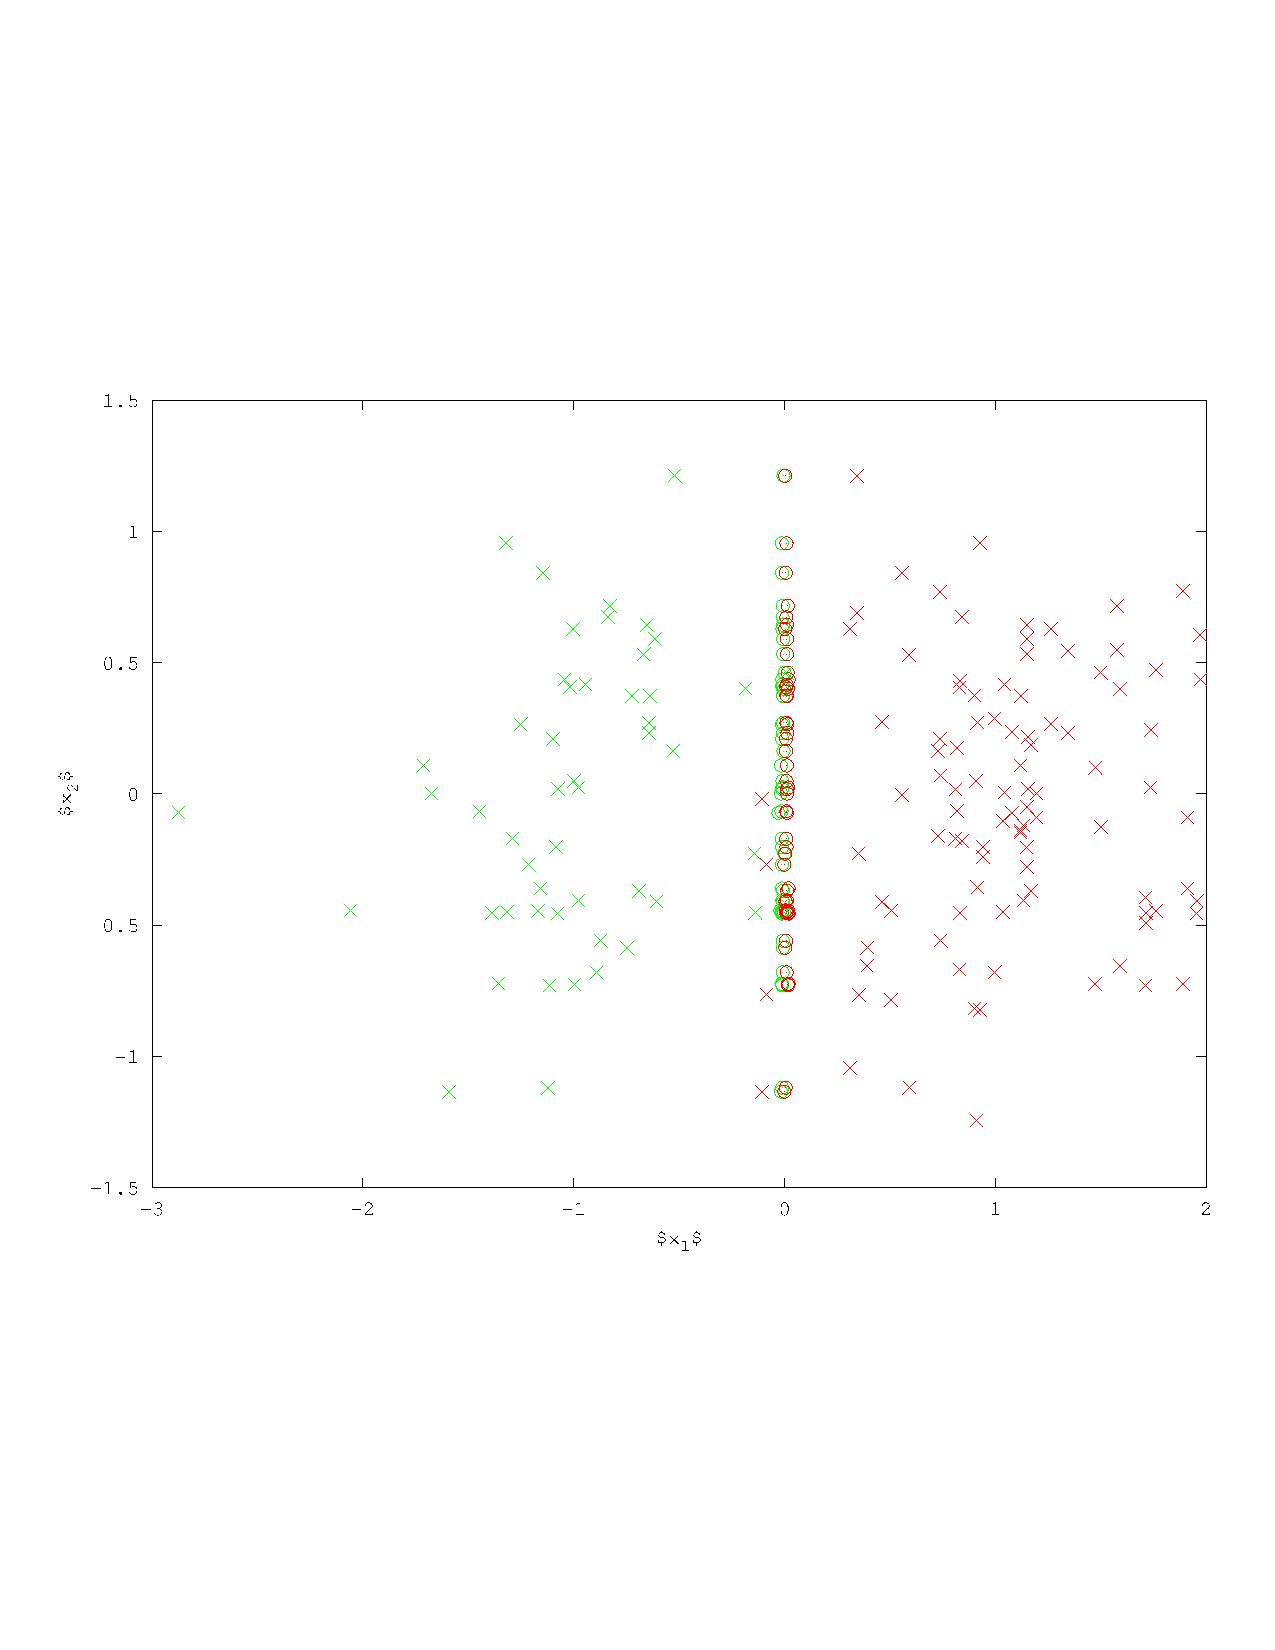
\includegraphics[width=.9\textwidth]{src/knollCdmetr.pdf}
  \captionof{figure}{Visualisation of the \knollC test set, before and after transforming it using \vect{M}}\label{fig:knollCd}
\end{minipage}
\hfill\\[.3em]

The error rates drop dramatically. This is because our metric ``spreads out'' the points along the $x_1$-axis, meaning that the nearest neighbours are more likely to be located along the $x_2$ axis instead of the $x_1$. One could also think of it as adding a penalty to the distance along the $x_1$ axis. This is important because the distance along the $x_1$ axis is actually what separates the two classes. We've visualised the effect of transforming \knollC test set using \vect{M} in fig.~\ref{fig:knollCd}.

\end{document}
